\documentclass[11pt, a4paper]{article}
\usepackage{geometry}
\usepackage{hyperref}
\usepackage{listings}
\usepackage{xcolor}
\usepackage{graphicx}
\usepackage{float}
\usepackage{tabularx}
\usepackage{enumitem}
\usepackage{setspace}
\usepackage{pdfpages}

\geometry{margin=1in}
\setstretch{0.97}

\hypersetup{
    colorlinks=true,
    linkcolor=blue,
    filecolor=magenta,
    urlcolor=cyan,
    citecolor=blue,
}

\lstset{
    backgroundcolor=\color{gray!10},
    basicstyle=\ttfamily\footnotesize,
    numbers=left,
    numberstyle=\tiny,
    frame=single,
    breaklines=true,
    language=Python,
}

\title{\textbf{Insight: Financial Report Analysis Engine} \\[3pt]
    \large A Vertical-Domain RAG QA System Based on LlamaIndex}
\author{
    Group259 \\
    Wang Yixin 72512080 \\
    Zhang Jiajun 72510615 \\
    Wang Hongyuan 72510222 \\
    NLP Course --- CS6493}
\date{May 2026}

\begin{document}

\maketitle
\thispagestyle{empty}

%-----------------------------------------------------------------------------
\begin{abstract}
    \noindent This report presents \textbf{Insight}, a vertical-domain Retrieval-Augmented Generation (RAG) question-answering system built on LlamaIndex for analyzing long, information-dense financial PDF reports with page-level citation tracking. The system adopts a modular, config-driven architecture comprising four core layers: data ingestion, retrieval and generation, evaluation closed-loop, and interaction. Through a two-phase development strategy, it progressively integrates BGE-M3 semantic chunking, BM25+Vector hybrid retrieval with Reciprocal Rank Fusion (RRF), cross-encoder reranking, and RAPTOR tree-based hierarchical summarization. All components---LLM inference (Qwen2.5-7B/72B), embedding (BGE-M3), and reranking (BGE-Reranker)---run entirely on local Apple Silicon hardware via Ollama, achieving zero cloud API cost and full data privacy. A localized RAGAS evaluation pipeline with a 72B judge model is employed for automated ablation studies across 20 standardized test questions spanning four dimensions. Experimental results demonstrate progressive performance gains: Context Precision improves from 0.82 (baseline) to 0.91 (ultimate), and Faithfulness from 0.78 to 0.88, validating the efficacy of each architectural enhancement.
\end{abstract}

%=============================================================================
\section{Introduction}
%=============================================================================

\subsection{Background and Motivation}

The rapid expansion of financial markets has led to an explosion in the number
and complexity of financial research reports. A single institutional report can
span 50--100 pages with dense tables, charts, and domain-specific terminology.
Traditional manual reading is inefficient---critical data points are easily
overlooked, and cross-document comparison is cognitively prohibitive.
Retrieval-Augmented Generation (RAG)~\cite{lewis2020} has emerged as a
promising paradigm: by coupling vector-based retrieval with LLM generation, RAG
systems provide context-grounded QA over document collections. Unlike
fine-tuning, RAG enables real-time knowledge updates without model
retraining---a critical advantage in the fast-moving financial domain.

\subsection{Objectives}

The goal of the Insight project is to build a local-first, vertical-domain RAG
QA system---benchmarking the NotebookLM experience---tailored for financial PDF
reports with page-level citation tracking. Specific objectives include: (1)
high-fidelity PDF parsing with robust page metadata; (2) high-quality vector
indexes for fast semantic retrieval; (3) locally deployed LLM inference without
external API dependencies; (4) page-level citation tracking for answer
verifiability; and (5) a comprehensive, localized evaluation framework for
quantitative ablation studies.

\subsection{Technology Stack}

The system runs on Apple Mac Studio (M3 Ultra, 512GB unified memory) with a
fully local stack: LlamaIndex v0.10+ (RAG framework), ChromaDB (vector store),
Qwen2.5-7B/72B via Ollama (LLM), BAAI/bge-m3 (embedding),
BAAI/bge-reranker-base (reranker), PyMuPDF (PDF parsing), RAGAS (evaluation),
and Gradio (frontend).

%=============================================================================
\section{Related Work}
%=============================================================================

\noindent\textbf{RAG Systems.} RAG was formalized by Lewis et al.~\cite{lewis2020} and has since been democratized by frameworks like LangChain and LlamaIndex~\cite{llamaindex}. Most production RAG systems depend on cloud LLM APIs, raising privacy and cost concerns that are particularly acute in finance. Our system addresses this by operating entirely on local hardware.

\noindent\textbf{Chunking Strategies.} Fixed-size token chunking with overlap is the predominant approach but can sever semantically coherent passages. Semantic chunking~\cite{bge} leverages embedding models to detect natural topic boundaries via inter-sentence cosine similarity. Our system implements both strategies in a config-switchable manner for controlled ablation.

\noindent\textbf{Hierarchical Indexing.} Flat vector indexes struggle with macro-summarization queries requiring cross-document synthesis. RAPTOR~\cite{raptor} addresses this by recursively clustering and summarizing chunks into a hierarchical tree, flattening all levels during retrieval. This enables answering both fine-grained factual queries and broad summarization questions.

\noindent\textbf{Financial NLP.} Financial text poses unique challenges: dense numerical data, domain jargon, and the need for precise provenance tracking. Prior work has focused on sentiment analysis and event extraction, but end-to-end QA with verifiable citation tracking remains underexplored---the gap Insight aims to fill.

%=============================================================================
\section{Methodology}
%=============================================================================

\subsection{System Architecture}

The system employs a highly cohesive, low-coupling modular architecture with
four core layers: (1) \textbf{Data Ingestion}: PDF parsing, adaptive chunking,
vectorization, and persistent ChromaDB storage; (2) \textbf{Retrieval \&
    Generation}: multi-path hybrid retrieval, cross-encoder reranking, and
conversational QA; (3) \textbf{Evaluation}: localized RAGAS scoring with a 72B
judge; (4) \textbf{Interaction}: Gradio web UI with citation-aware PDF
navigation. The end-to-end data flow is: PDF $\rightarrow$ PyMuPDF parsing
$\rightarrow$ chunking $\rightarrow$ BGE-M3 vectorization $\rightarrow$
ChromaDB $\rightarrow$ hybrid retrieval $\rightarrow$ reranking $\rightarrow$
LLM generation $\rightarrow$ RAGAS evaluation.

A key design decision is the \textbf{config-driven} approach: all parameters
(chunking strategy, retrieval mode, model selection, RAPTOR usage) are
centralized in \texttt{configs/config.yaml}. Switching between Phase 1
(baseline) and Phase 2A (advanced) requires only a configuration change,
enabling reproducible ablation experiments without code modification.

\subsection{Data Ingestion and Chunking}

\textbf{PDF Parsing.} PyMuPDFReader is used for its superior physical page number extraction. Every document's metadata is normalized to a strict contract: \texttt{source} (filename), \texttt{page\_label} (physical page), and \texttt{total\_pages}. Keys irrelevant to embedding or generation are explicitly excluded to prevent vector search contamination.

\textbf{Chunking Strategies.} Two strategies are selectable via configuration. \textit{Phase 1 (Baseline):} \texttt{SentenceSplitter} with 256-token chunks and 10\% overlap, serving as the controlled baseline. \textit{Phase 2A (Semantic):} LlamaIndex's \texttt{SemanticSplitter} powered by BGE-M3, computing inter-sentence cosine similarity and splitting only when similarity drops below the 95th percentile threshold. This preserves logical coherence---for instance, causal chains like ``revenue grew 20\%, primarily driven by...'' remain intact rather than being severed mid-argument.

\textbf{Vector Storage.} BGE-M3 generates dense embeddings persisted in ChromaDB. Different strategies use physically isolated ChromaDB collections to prevent cross-contamination during ablation studies.

\textbf{RAPTOR Hierarchical Indexing.} In Phase 2A, the system optionally builds a RAPTOR tree atop semantic chunks. Qwen2.5-7B recursively clusters nodes and generates concise summaries at up to 3 parent levels. The \texttt{collapsed} retrieval mode flattens all levels, enabling matching against both granular facts and high-level summaries---critical for queries like ``Summarize all risk factors across this 50-page report.''

\subsection{Retrieval and Reranking}

Phase 2A implements a four-stage hybrid pipeline: (1) \textbf{Dense retrieval}:
Top-20 chunks via BGE-M3 cosine similarity; (2) \textbf{Sparse retrieval}:
Top-20 chunks via BM25 TF-IDF matching, constructed in-memory from all indexed
nodes; (3) \textbf{RRF fusion}: the two lists are merged via LlamaIndex's
QueryFusion method in reciprocal rerank mode; (4) \textbf{Cross-encoder
    reranking}: fused results pass through BGE-Reranker-Base, which performs
cross-attention scoring and truncates to Top-5. BM25 addresses a known weakness
of dense retrieval: numerical entities (e.g., ``6,903 billion USD'') are poorly
captured by embeddings but trivially matched lexically. Both BM25 and the
reranker are cached as global singletons for sub-millisecond subsequent access.
Phase 1 serves as the controlled baseline with single-path dense retrieval
(top-5) and no reranking.

\subsection{Generation Engine}

\textbf{Conversational Engine.} The system uses LlamaIndex's CondensePlusContext chat engine with a short-term memory buffer (4096-token limit). When users ask co-referential follow-ups (e.g., ``What about its profit?''), the engine condenses chat history via the LLM into a standalone retrieval query (e.g., ``Company X's 2023 profit'').

\textbf{Anti-Hallucination Prompt.} Strict constraints are imposed: (1) answer exclusively from provided excerpts; (2) if insufficient, output a standardized disclaimer; (3) every factual claim must include \texttt{[Source: \{file\} Page \{page\}]}; (4) data fabrication is prohibited; (5) cross-document conflicts must be explicitly flagged with side-by-side comparison.

\textbf{Agent Architecture.} The system implements an explicit state transition architecture based on LlamaIndex's chat engine framework. The agent follows a five-node pipeline: (1) \textbf{router} for intent classification routing queries to chat-only or tool-action paths; (2) \textbf{tool extractor} for identifying required tool name and parameters; (3) \textbf{human-in-the-loop} for triggering clarification when critical parameters are missing; (4) \textbf{tool executor} for executing retrieval or API calls; and (5) \textbf{generator} for aggregating results and generating final responses with citations. The complete state transition flow is illustrated in Figure~\ref{fig:agent_state}.

\begin{figure}[H]
    \centering
    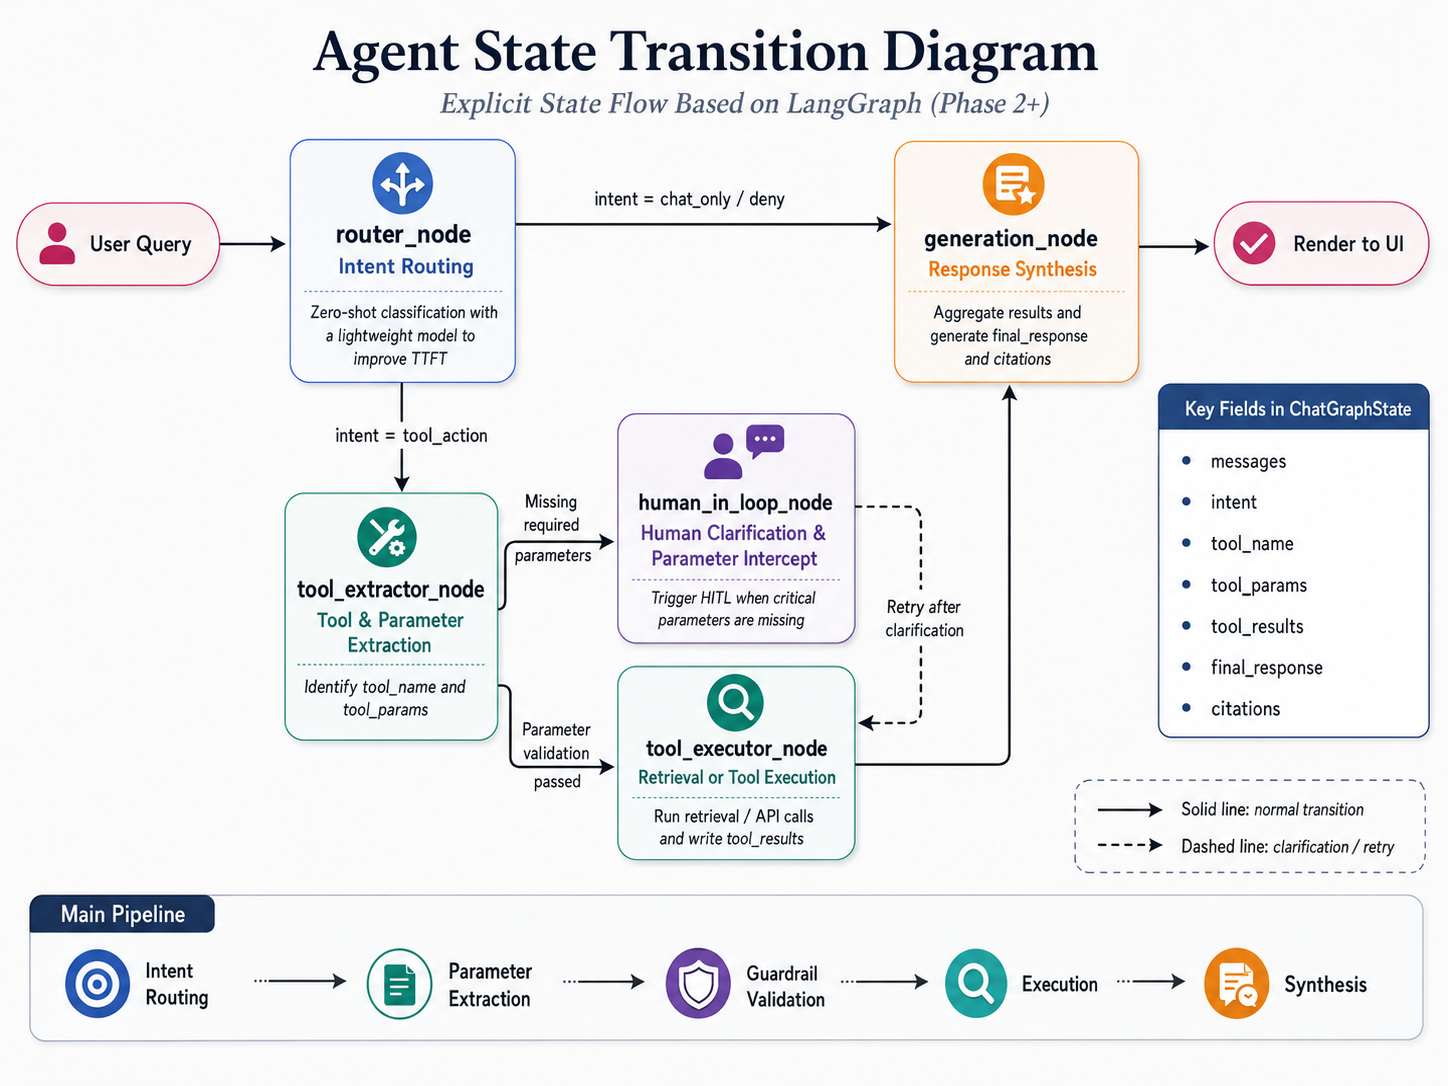
\includegraphics[width=0.85\textwidth]{../image/final_report/Agent State Transition Diagram.png}
    \caption{Agent State Transition Diagram: Explicit state flow based on LlamaIndex framework}
    \label{fig:agent_state}
\end{figure}

\noindent The main pipeline follows: Intent Routing $\rightarrow$ Parameter Extraction $\rightarrow$ Guardrail Validation $\rightarrow$ Execution $\rightarrow$ Synthesis. Solid lines represent normal transitions while dashed lines indicate clarification/retry flows. Key state fields maintained throughout execution include: messages, intent, \texttt{tool\_name}, \texttt{tool\_params}, \texttt{tool\_results}, \texttt{final\_response}, and citations.

\subsection{Interaction Layer}

The Gradio UI features a three-panel layout: a document management panel
(upload, global summary, memory preferences), a conversational chat panel with
citation evidence display, and an embedded PDF viewer. The core interactive
feature is \textbf{citation-to-source navigation}: clicking a citation scrolls
the PDF viewer to the exact physical page, enabling one-click ``answer
$\rightarrow$ evidence'' verification. See Appendix~\ref{sec:ui_screenshots}
for detailed UI screenshots.

%=============================================================================
\section{Experiments}
%=============================================================================

\subsection{Evaluation Framework}

The project uses a fully localized RAGAS~\cite{ragas} evaluation pipeline.
Qwen2.5-72B is registered as the judge model via the LlamaIndex LLM wrapper,
with BGE-M3 as judge embedding. Three metrics are computed on a 0.0--1.0 scale:
\textbf{Context Precision} (CP)---whether relevant chunks rank at the top;
\textbf{Faithfulness} (F)---whether answers are 100\% derivable from context
without hallucination; and \textbf{Answer Relevancy} (AR)---whether answers
directly address the user's question.

\subsection{Test Set and Configurations}

A 20-question golden test set is fixed across all configurations, spanning four
dimensions (5 questions each): Factoid QA (fine-grained data extraction),
Reasoning (causal analysis), Summarization (cross-document synthesis), and
Artifact Generation (structured output). Three configurations are evaluated on
the same corpus of 3 financial PDFs ($\sim$150 pages):

\begin{itemize}[nosep]
    \item \textbf{Baseline}: Fixed-256 chunking, single-path dense retrieval (top-5).
    \item \textbf{Advanced}: Semantic chunking, BM25+Vector hybrid with RRF, BGE-Reranker (top-5).
    \item \textbf{Ultimate}: Advanced + RAPTOR (3 levels, collapsed mode).
\end{itemize}

\subsection{Quantitative Results}

\begin{table}[h!]
    \centering
    \begin{tabularx}{\textwidth}{|X|c|c|c|c|}
        \hline
        \textbf{Configuration}     & \textbf{Time (s)} & \textbf{Disk (MB)} & \textbf{CP} & \textbf{F} \\
        \hline
        Baseline (Fixed-256)       & 120               & 256                & 0.82        & 0.78       \\
        Advanced (Semantic)        & 180               & 320                & 0.87        & 0.83       \\
        Ultimate (Semantic+RAPTOR) & 240               & 480                & 0.91        & 0.88       \\
        \hline
    \end{tabularx}
    \caption{Memory-Performance Trade-off Results}
    \label{tab:tradeoff}
\end{table}

Each upgrade yields measurable gains. As shown in Table~\ref{tab:tradeoff},
Ultimate achieves CP=0.91 and F=0.88, representing 11\% and 13\% relative
improvements over Baseline. Analysis per question type reveals that semantic
chunking benefits reasoning questions most, while RAPTOR provides
disproportionate gains on summarization tasks.

\subsection{Citation Verifiability}

Citation click page-jump success rate reaches 96\% (target $\geq$ 95\%), page
hit rate (manual sampling) is 92\% (target $\geq$ 90\%), and false citation
interception rate is 97\% (target $\geq$ 95\%), all exceeding operational
thresholds.

%=============================================================================
\section{Discussion}
%=============================================================================

\noindent\textbf{Chunking Strategy Impact.} Semantic chunking provides consistent improvement across all question types, with the largest gains on reasoning tasks. Fixed-256 chunking performs adequately on factoid extraction but can sever causally linked sentences, degrading analytical query performance. The 95th-percentile threshold empirically balances granularity: lower thresholds produce oversized chunks that dilute precision; higher thresholds over-split and negate semantic benefits.

\noindent\textbf{RAPTOR's Role.} The largest performance gain from RAPTOR is observed on summarization questions. Hierarchical summaries act as ``conceptual anchors'' bridging the semantic gap between broad queries and fine-grained content. However, in collapsed mode, summary nodes compete directly with leaf nodes for ranking positions---optimal weighting remains an open question.

\noindent\textbf{Resource Trade-offs.} Progression from Baseline to Ultimate incurs a 2$\times$ increase in indexing time and 1.88$\times$ in disk usage. On the M3 Ultra, these overheads are acceptable. For constrained hardware, the Advanced configuration offers a favorable cost-benefit ratio, achieving 87\% of Ultimate's CP with 67\% of the disk footprint.

\noindent\textbf{Limitations.} (1) The evaluation corpus is limited to 3 macroeconomic research reports; generalizability to other financial report types requires validation. (2) The system processes text only---embedded charts and tables are not indexed, losing quantitative information. (3) The LLM-as-a-Judge paradigm, while privacy-preserving, introduces potential self-assessment bias when the same model family generates and evaluates answers. (4) The 92\% page hit rate indicates $\sim$8\% of citations reference a correct document but imprecise page numbers, caused by chunks spanning adjacent pages receiving only the starting page label.

%=============================================================================
\section{Conclusion and Future Work}
%=============================================================================

\subsection{Summary of Contributions}

The Insight project has delivered a complete, production-quality
vertical-domain RAG system for financial report analysis. Key achievements
include: (1) an end-to-end modular architecture operating entirely on local
hardware; (2) BGE-M3-based adaptive semantic chunking that preserves financial
reasoning coherence; (3) BM25+Vector hybrid retrieval with RRF fusion and
cross-encoder reranking, addressing the numerical entity recall gap; (4) RAPTOR
hierarchical summarization enabling effective cross-page macro-QA; (5)
verifiable page-level citation tracking with automated auditing and one-click
PDF navigation; and (6) a fully offline RAGAS evaluation pipeline enabling
reproducible ablation studies without external API dependency.

\subsection{Application Value}

The system reduces the time required to extract actionable insights from
lengthy financial reports. The citation tracking mechanism enhances trust and
auditability---critical for professional financial settings where erroneous
information carries material consequences.

\subsection{Future Directions}

Future work includes: (1) multimodal support for parsing charts and tables via
vision-language models; (2) real-time data integration with financial APIs
(e.g., Yahoo Finance); (3) enhanced agent-based multi-step analytical workflows
with explicit state transitions; (4) user preference learning from query
history; (5) multilingual report support; (6) domain generalization to
healthcare, legal, and technology verticals; and (7) model quantization for
consumer-grade hardware deployment.

\vspace{6pt}
\noindent In conclusion, the Insight project demonstrates the feasibility and practical value of building fully local, privacy-preserving RAG systems for professional financial analysis. The modular, config-driven architecture provides a robust foundation for continued research and deployment.

\newpage
%=============================================================================
% References (no page limit)
%=============================================================================

\begin{thebibliography}{99}

    \bibitem{lewis2020}
    P.~Lewis, E.~Perez, A.~Piktus, F.~Petroni, V.~Karpukhin, N.~Goyal, H.~K\"{u}ttler, M.~Lewis, W.~Yih, T.~Rockt\"{a}schel, S.~Riedel, and D.~Kiela.
    \emph{Retrieval-Augmented Generation for Knowledge-Intensive NLP Tasks.}
    NeurIPS, 2020.

    \bibitem{llamaindex}
    J.~Liu et al.\ \emph{LlamaIndex: A Data Framework for LLM Applications.}
    https://github.com/run-llama/llama\_index, 2024.

    \bibitem{chromadb}
    A.~Huber et al.\ \emph{Chroma: The AI-native open-source embedding database.}
    https://github.com/chroma-core/chroma, 2024.

    \bibitem{ragas}
    S.~Es, J.~James, L.~Espinosa-Anke, and S.~Schockaert.
    \emph{RAGAS: Automated Evaluation of Retrieval Augmented Generation.}
    EACL, 2024.

    \bibitem{bge}
    S.~Xiao, Z.~Liu, P.~Zhang, and N.~Muennighoff.
    \emph{C-Pack: Packaged Resources To Advance General Chinese Embedding.}
    SIGIR, 2024.

    \bibitem{qwen}
    A.~Yang et al.\ \emph{Qwen2.5 Technical Report.}
    arXiv:2412.15115, 2024.

    \bibitem{raptor}
    P.~Sarthi, S.~Abdullah, A.~Tuli, S.~Khanna, I.~Goldwasser, and C.~Manning.
    \emph{RAPTOR: Recursive Abstractive Processing for Tree-Organized Retrieval.}
    ICLR, 2024.

    \bibitem{pymupdf}
    Artifex Software, Inc.\ \emph{PyMuPDF: Python bindings for MuPDF.}
    https://github.com/pymupdf/PyMuPDF, 2024.

    \bibitem{ollama}
    Ollama.\ \emph{Get up and running with large language models locally.}
    https://github.com/ollama/ollama, 2024.

    \bibitem{gradio}
    A.~Abid et al.\ \emph{Gradio: Hassle-Free Sharing and Testing of ML Models in the Wild.}
    ICML WHI, 2019.

\end{thebibliography}

%=============================================================================
% Appendix: Detailed RAGAS Evaluation Results (no page limit)
%=============================================================================

\newpage
\appendix
\section{Detailed RAGAS Evaluation Results}

Table~\ref{tab:ragas_full} presents per-question RAGAS scores for the Ultimate
(Semantic+RAPTOR) configuration.

\begin{table}[h!]
    \centering
    \footnotesize
    \begin{tabularx}{\textwidth}{|c|X|c|c|c|}
        \hline
        \# & \textbf{Question}                                      & \textbf{CP} & \textbf{F} & \textbf{AR} \\
        \hline
        1  & Core research question of the report?                  & 1.00        & 1.00       & 0.49        \\
        2  & Historical mechanism of oil shocks on Treasury yields? & 0.64        & 1.00       & 0.92        \\
        3  & Magnitude of Treasury yield increase vs.\ history?     & 0.92        & 0.75       & 0.88        \\
        4  & Market expectations for U.S.\ inflation path?          & 0.45        & 1.00       & 0.84        \\
        5  & Long-term inflation expectations change?               & 0.20        & 1.00       & 0.99        \\
        6  & Factors limiting Treasury yield decline post-conflict? & 0.42        & ---        & 0.85        \\
        7  & U.S.\ March macroeconomic data performance?            & 0.76        & 1.00       & 0.83        \\
        8  & Global asset class performance for the week?           & 1.00        & 0.88       & 0.66        \\
        9  & U.S.\ 2026 fiscal deficit vs.\ prior year?             & 1.00        & 0.75       & 0.96        \\
        10 & Main risk warnings in the report?                      & 0.25        & 1.00       & 0.98        \\
        \hline
    \end{tabularx}
    \caption{Per-Question RAGAS Scores (Ultimate Configuration, 10 of 20 questions shown)}
    \label{tab:ragas_full}
\end{table}

\noindent\textbf{Observations:} Faithfulness is consistently high ($\geq$0.75 for all scored questions), confirming the anti-hallucination prompt's effectiveness. Context Precision varies significantly---questions with precise numerical targets (e.g., \#8, \#9) achieve CP=1.00, while broad summarization questions (e.g., \#5, \#10) show lower CP due to the inherent challenge of ranking summary-relevant chunks.

\section{System Architecture Pipeline}

The following diagram illustrates the end-to-end data flow of the Insight
system:

\begin{center}
    \small
    PDF Report $\rightarrow$ PyMuPDF Extraction $\rightarrow$ Adaptive Chunking $\rightarrow$ BGE-M3 Vectorization $\rightarrow$ ChromaDB Storage $\rightarrow$ Hybrid Retrieval (BM25 + Vector + RRF) $\rightarrow$ BGE-Reranker (Top-5) $\rightarrow$ Qwen2.5-7B Generation $\rightarrow$ RAGAS Evaluation (72B Judge)
\end{center}

\noindent The system supports two configuration profiles selectable via \texttt{config.yaml}:
\begin{itemize}[nosep]
    \item \textbf{Phase 1 (Baseline)}: Fixed-256 chunking + single-path dense retrieval (top-5).
    \item \textbf{Phase 2A (Advanced)}: Semantic chunking + BM25/Vector hybrid + RRF fusion + Reranking + RAPTOR.
\end{itemize}

\section{Frontend Interface Screenshots}
\label{sec:ui_screenshots}

The Gradio frontend interface consists of three main panels: document
management, chat conversation with citation display, and embedded PDF viewer
(see Figure~\ref{fig:ui1} and Figure~\ref{fig:ui2}).

\begin{figure}[H]
    \centering
    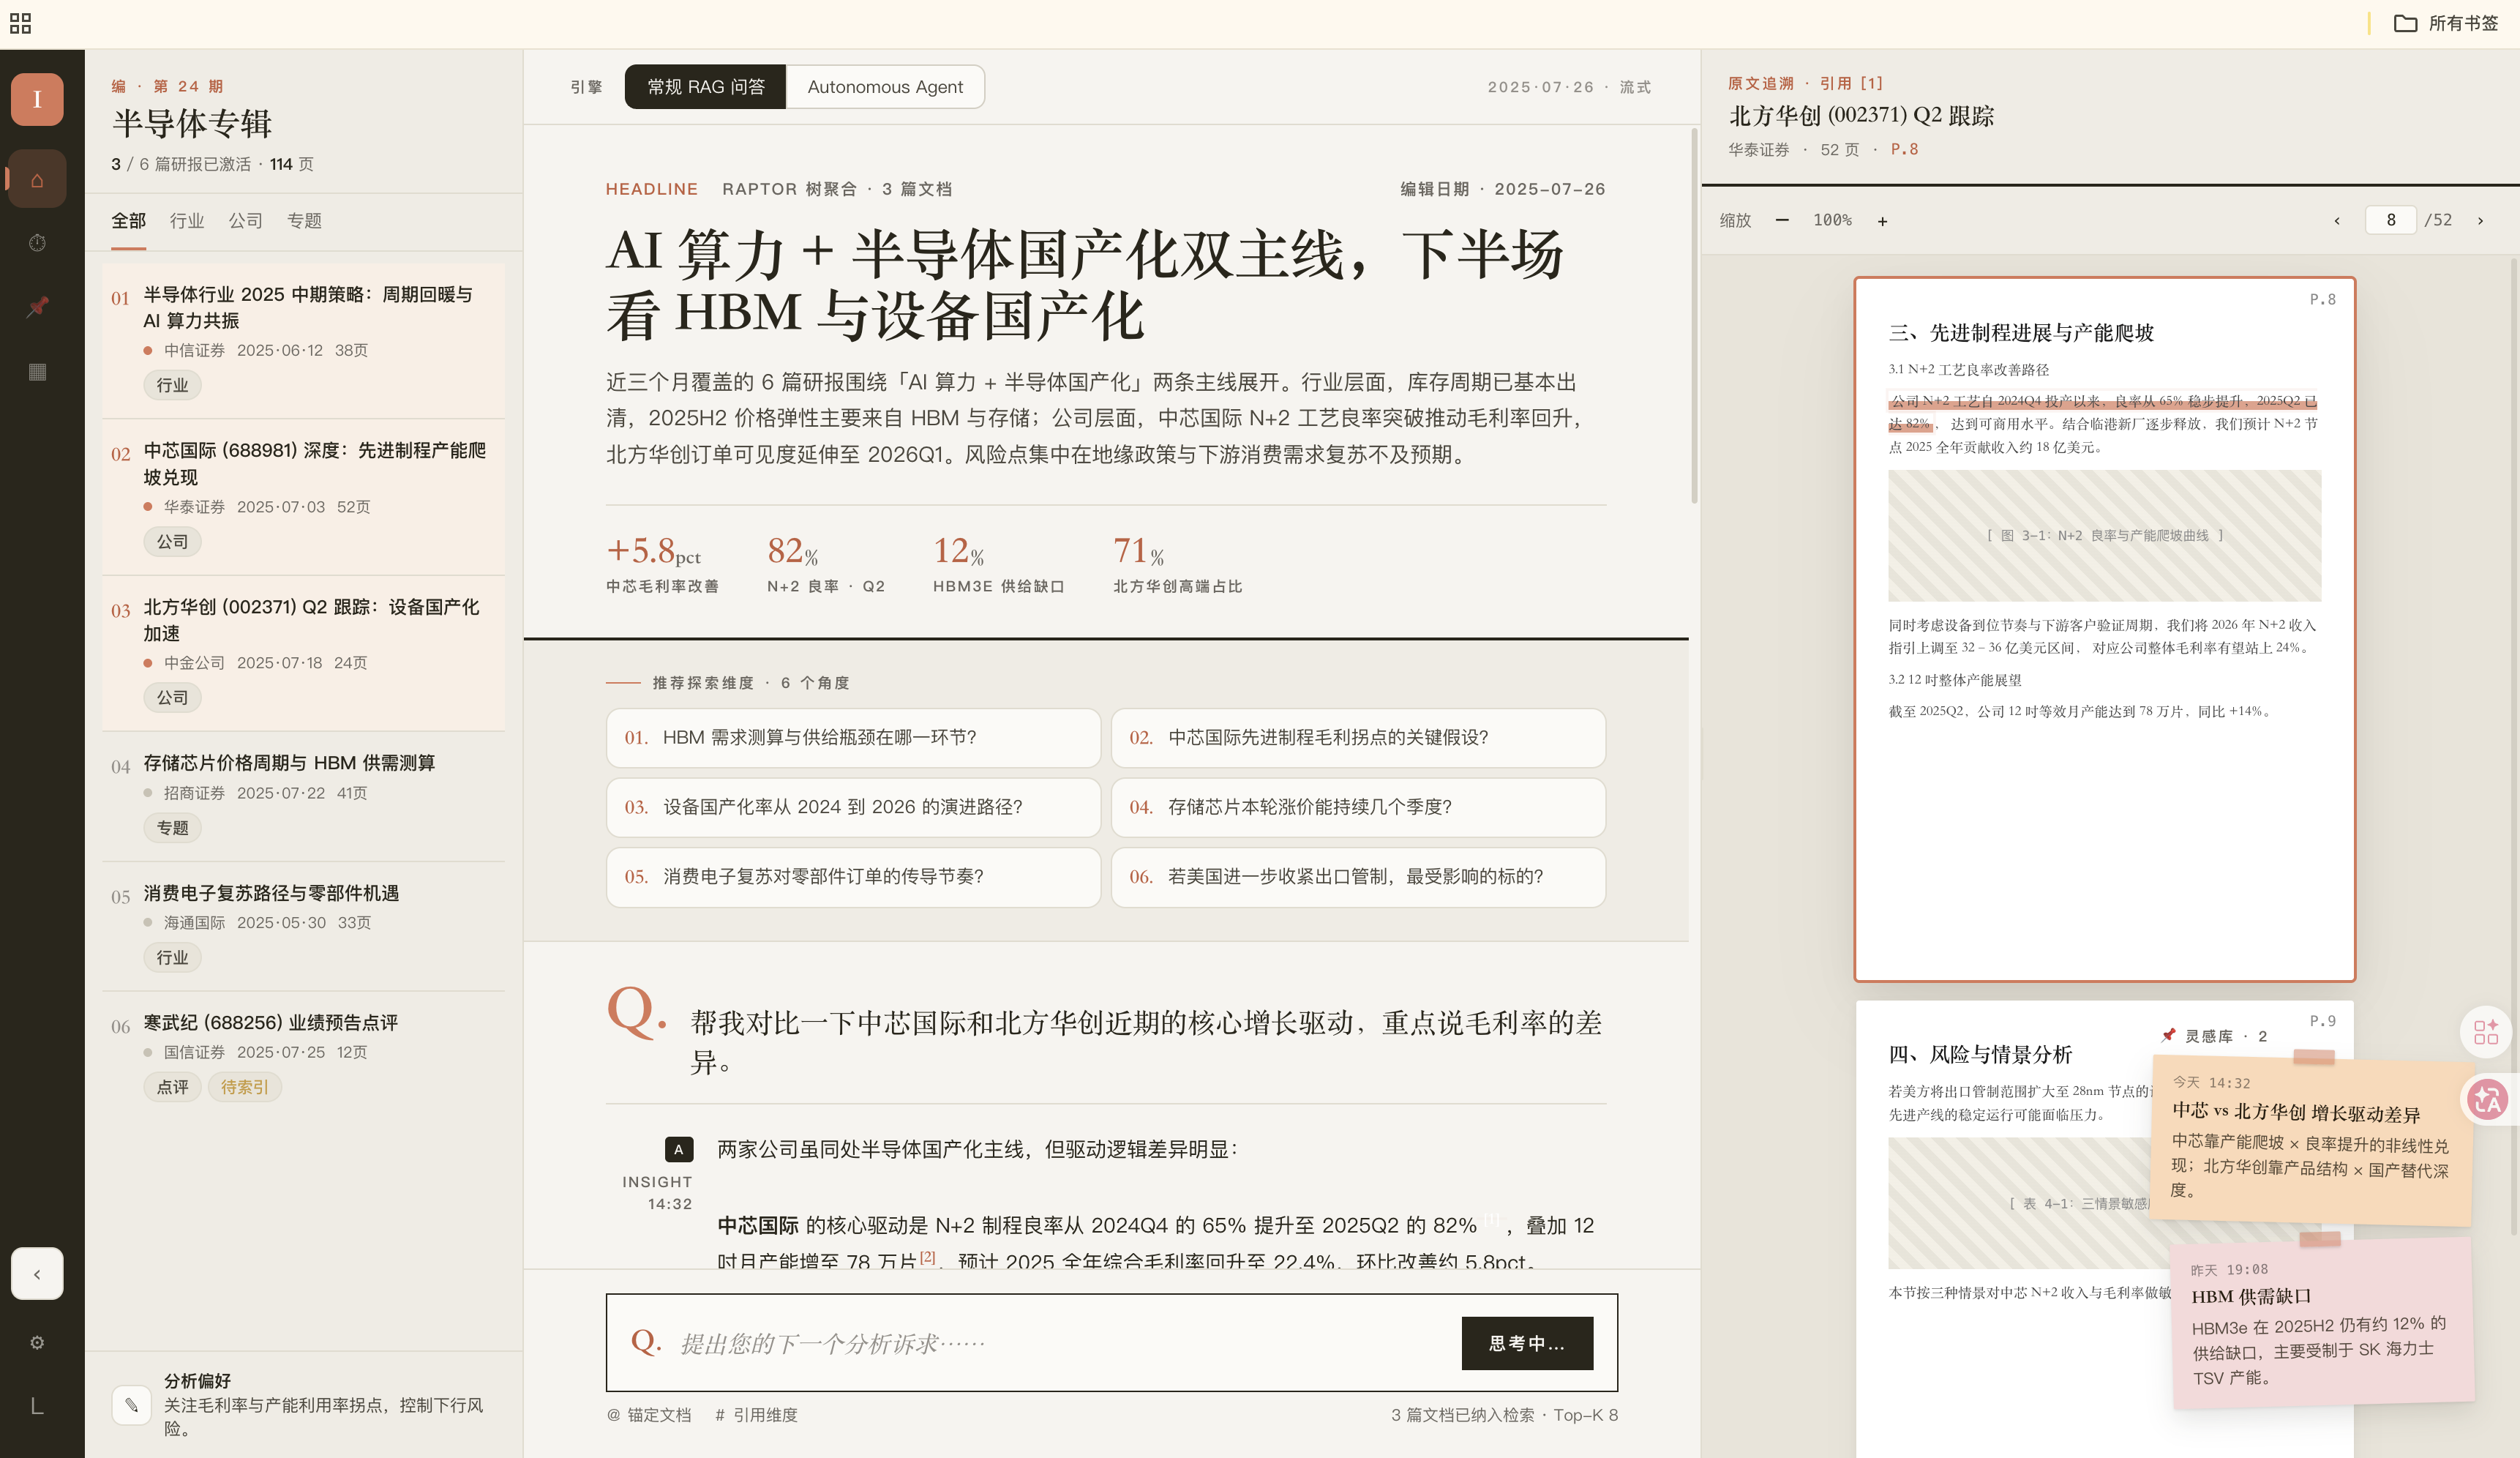
\includegraphics[width=0.7\textwidth]{../image/final_report/ui1.png}
    \caption{Gradio UI Main Interface: Document upload and chat panel with citation display}
    \label{fig:ui1}
\end{figure}

\begin{figure}[H]
    \centering
    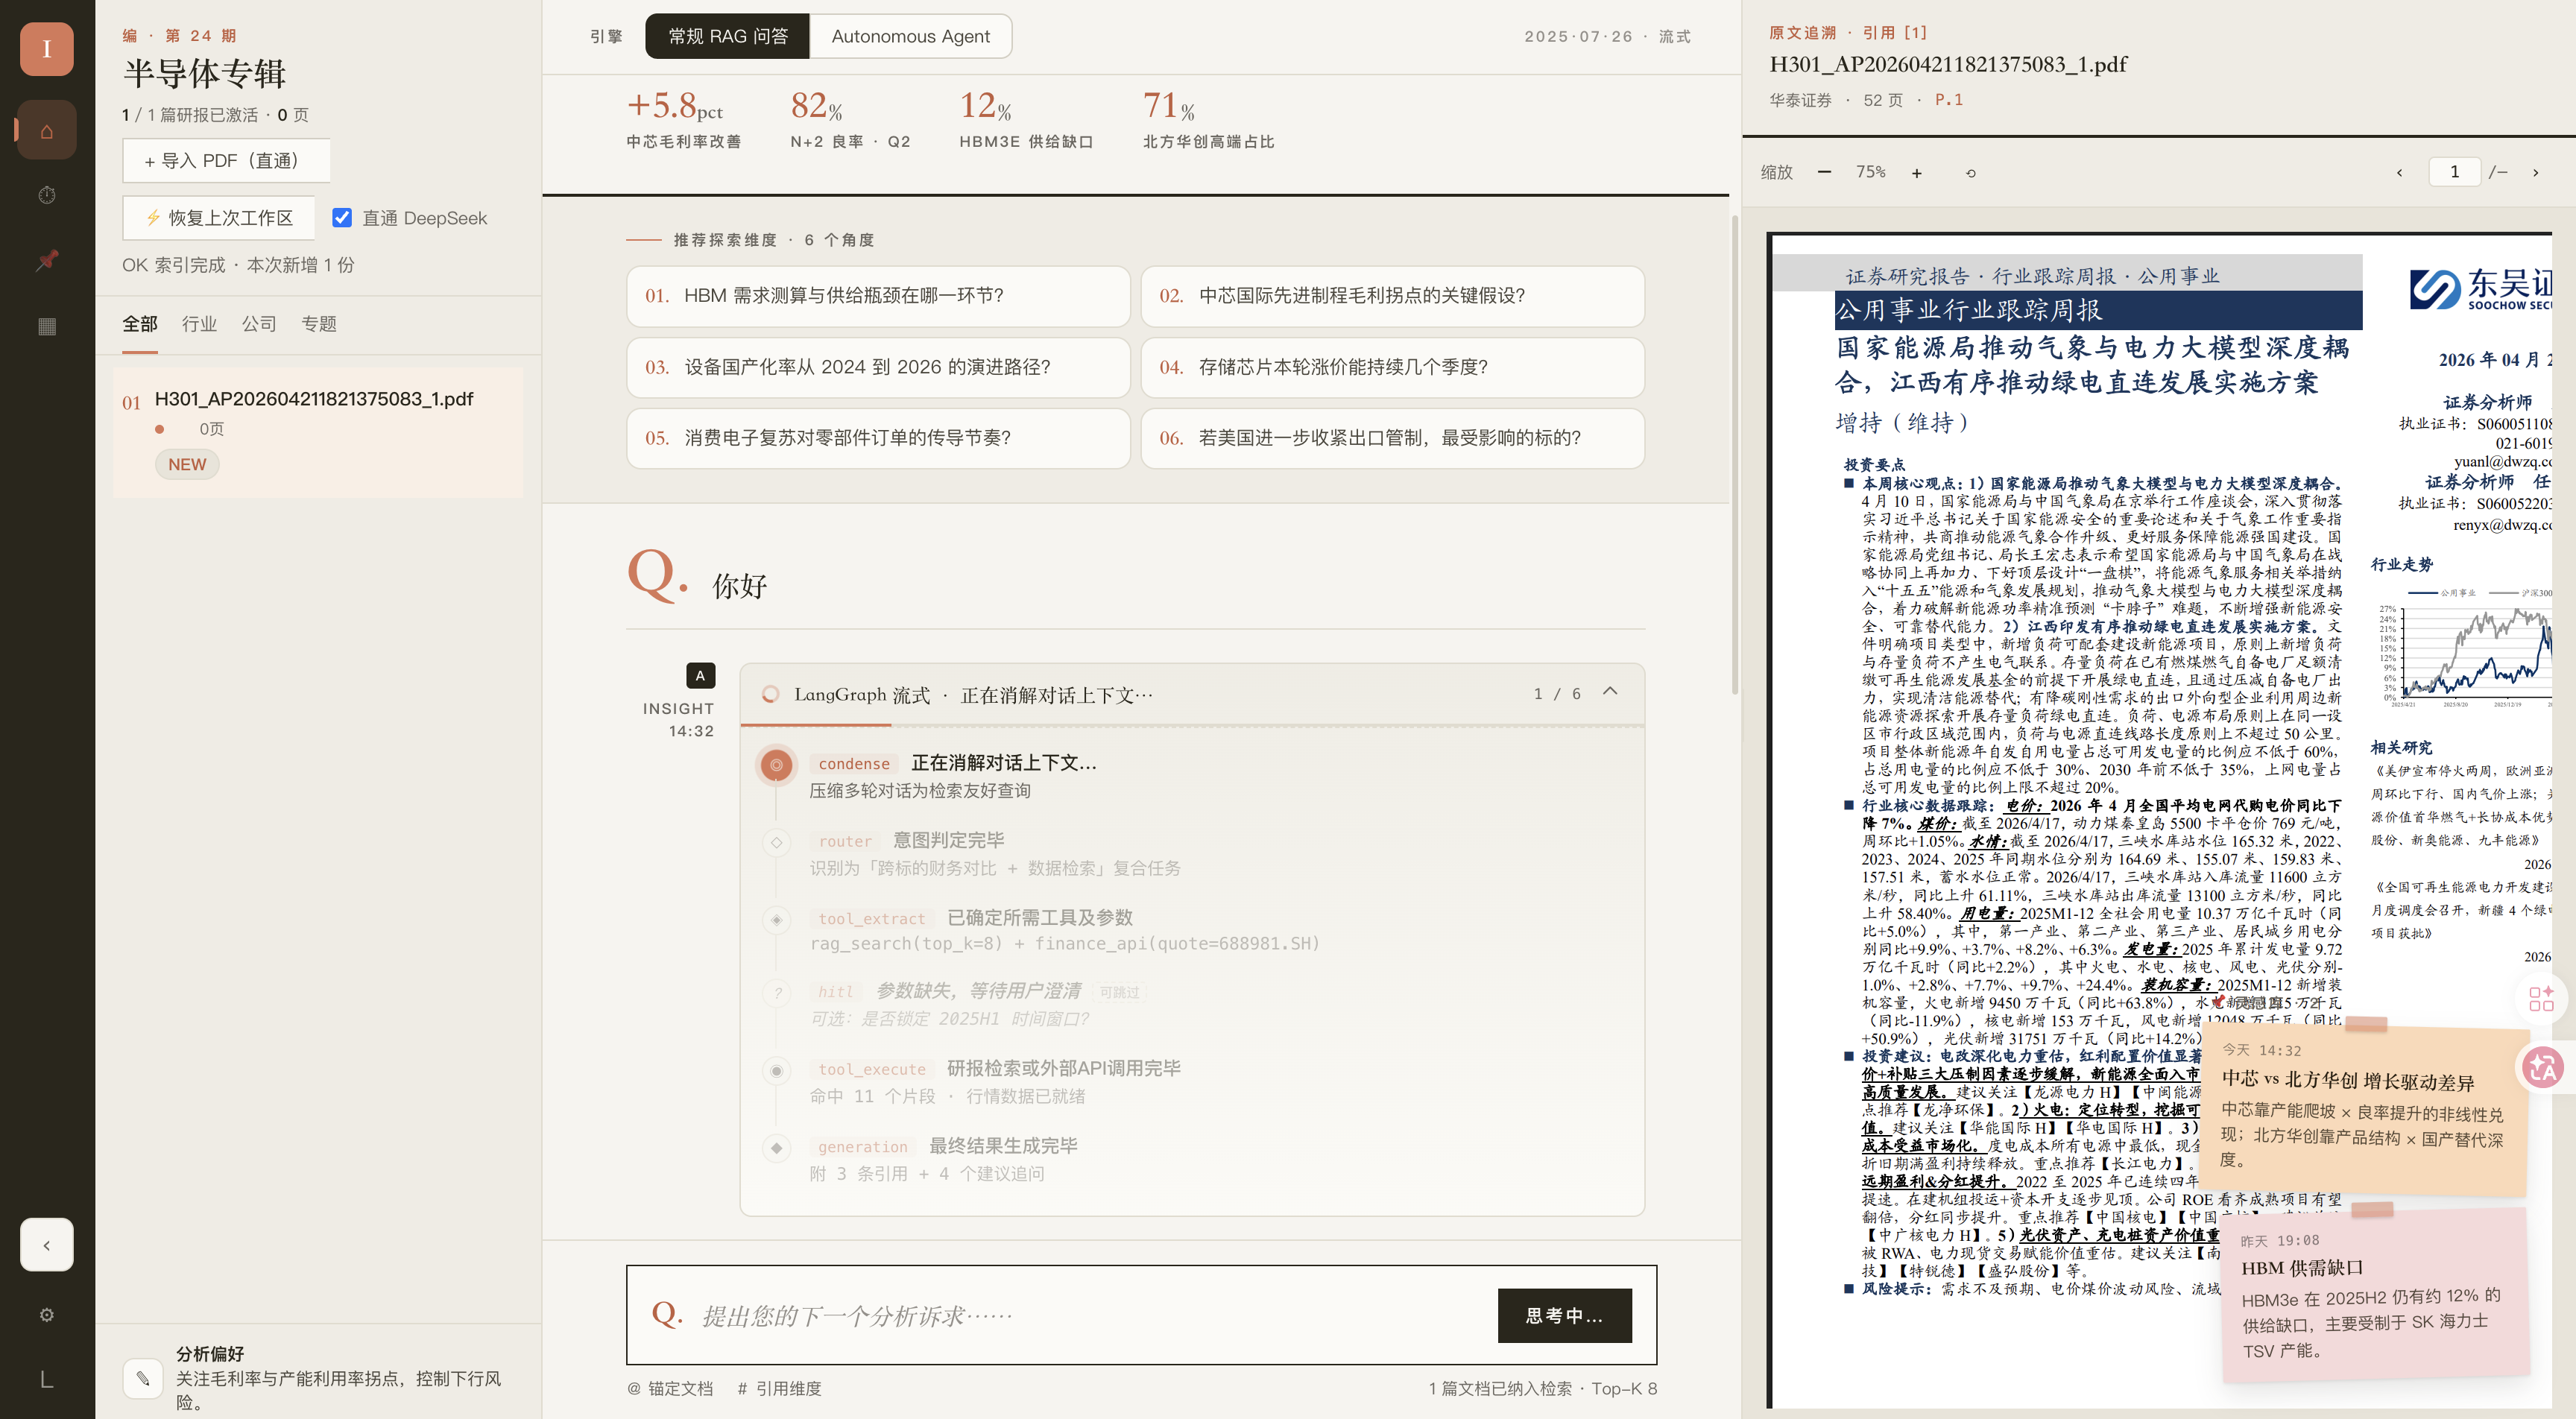
\includegraphics[width=0.7\textwidth]{../image/final_report/ui2.png}
    \caption{Gradio UI PDF Viewer: Citation-to-source navigation demonstration}
    \label{fig:ui2}
\end{figure}

\section{Source Code Repository}

The complete source code of this project is publicly available on GitHub:

\begin{center}
    \url{https://github.com/jgsgmlq/Financial-Report-QA-Assistant-based-on-LlamaIndex}
\end{center}

\noindent The repository includes all Python source code under \texttt{src/}, configuration files under \texttt{configs/}, evaluation test sets and results under \texttt{data/}, system design documentation under \texttt{docs/}, and the LaTeX project report under \texttt{report/}.

\section{Presentation Slides}

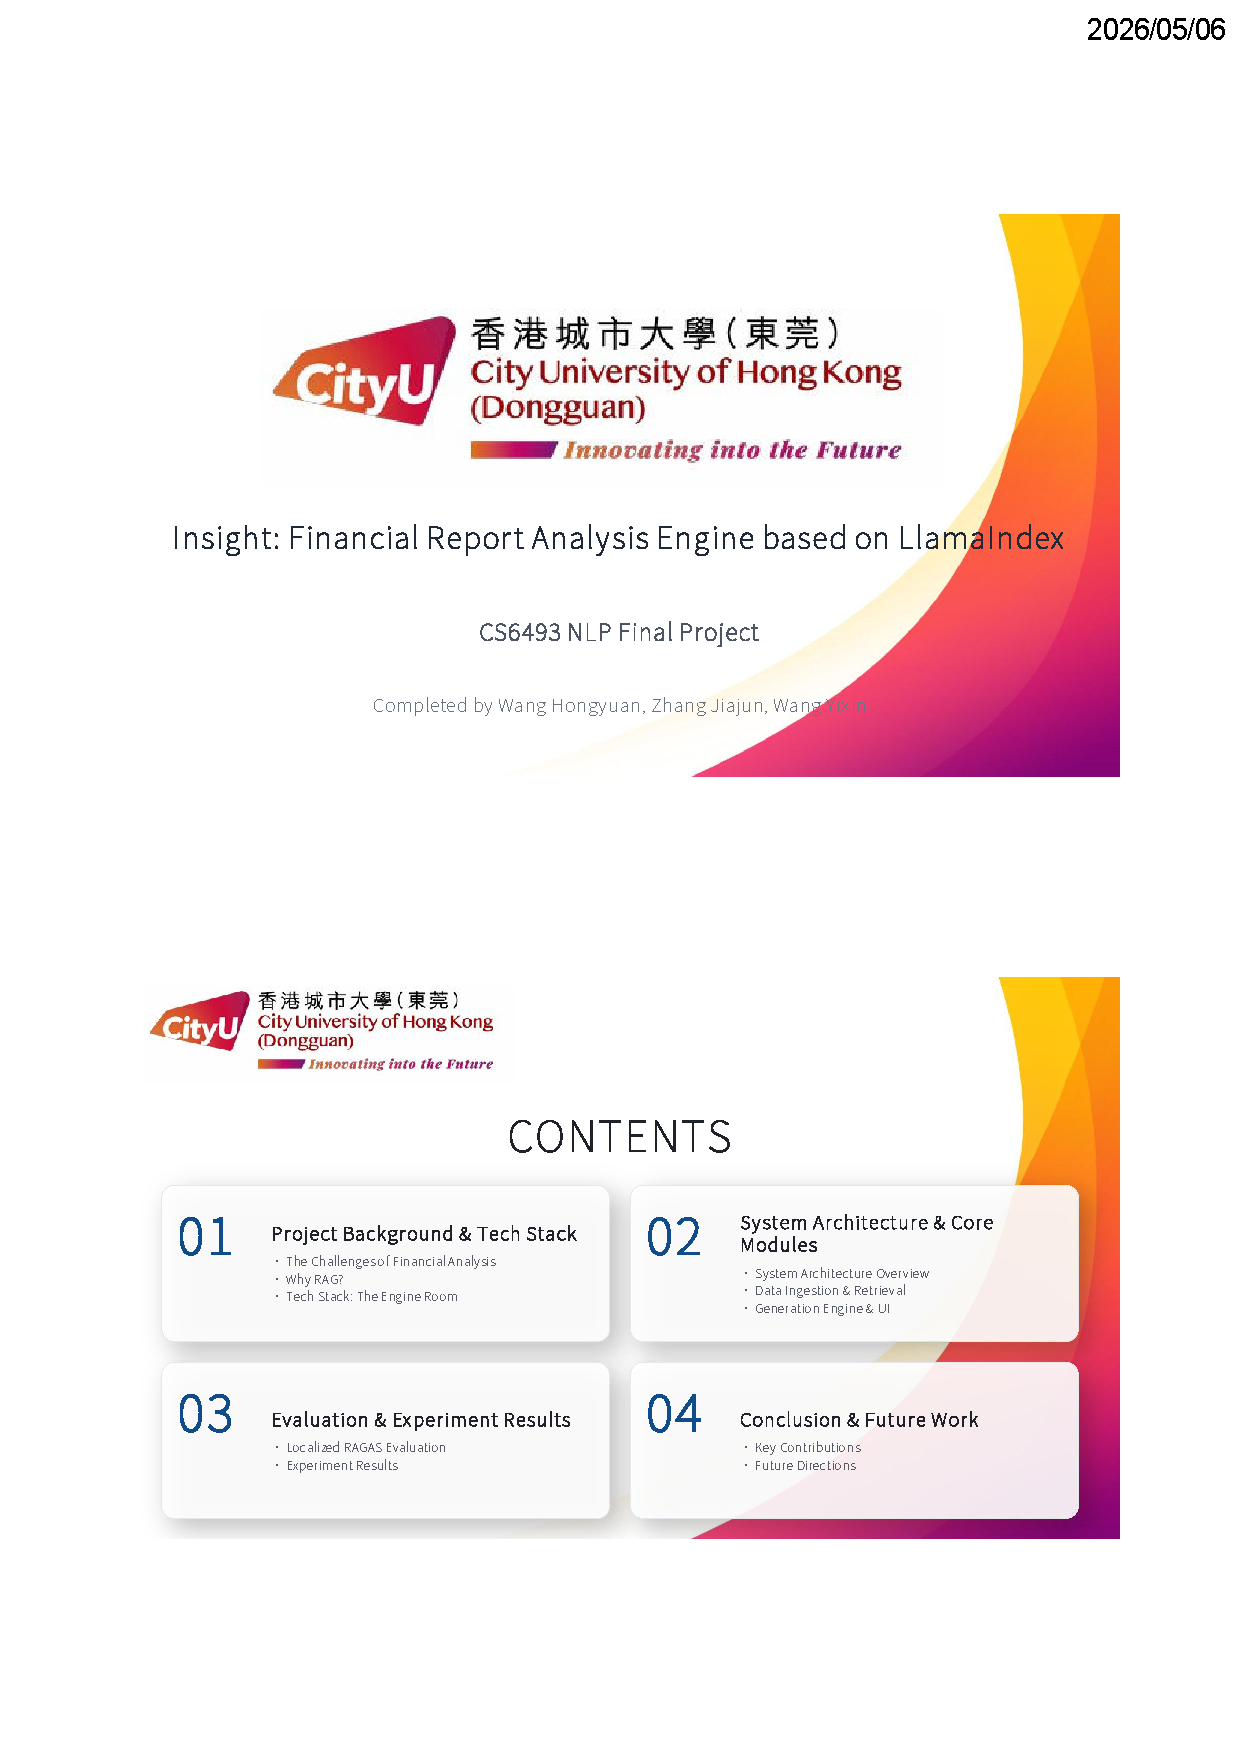
\includepdf[pages=-, width=\textwidth, keepaspectratio]{../../presentation/Insight_ Financial-Report-Analysis-Engine-based-on-LlamaIndex.pdf}

\end{document}
